\begin{frame}
    \frametitle{Learning algorithms - Asymmetric replicator dynamics}

    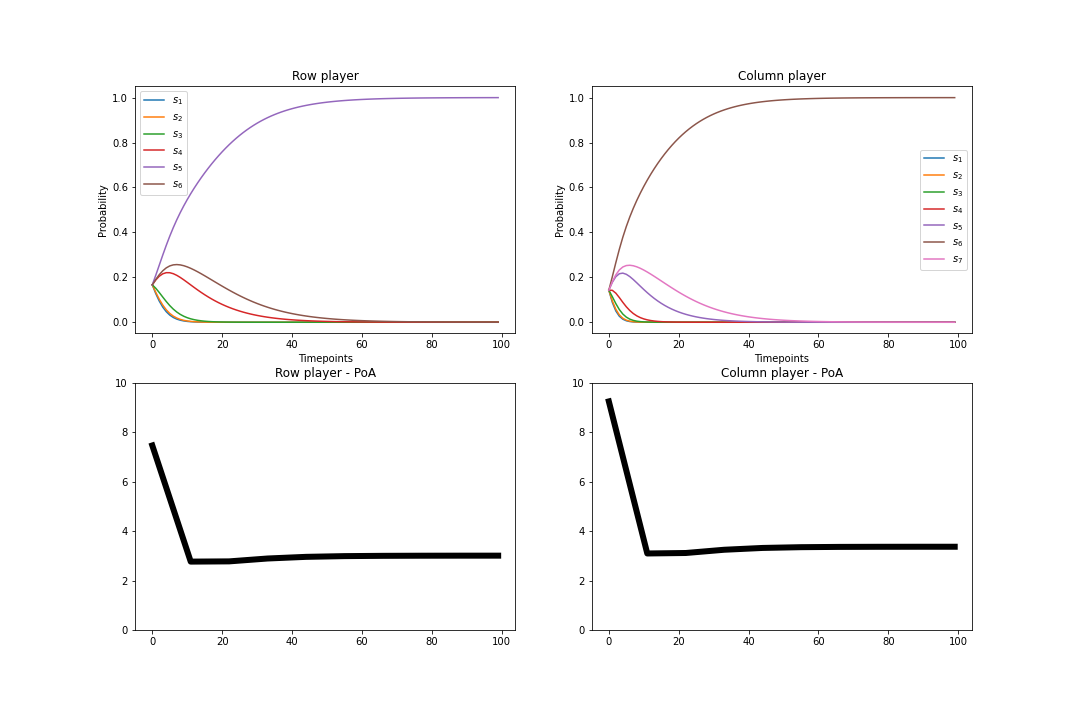
\includegraphics[scale=0.28]{Bin/ARD_game.png}
    
\end{frame}

\begin{frame}
    \centering
    \Huge{
    ``Inefficiencies can be learned and emerged naturally in an interactive system''
    }
\end{frame}


\begin{frame}
    \frametitle{Learning algorithms - Asymmetric replicator dynamics}

    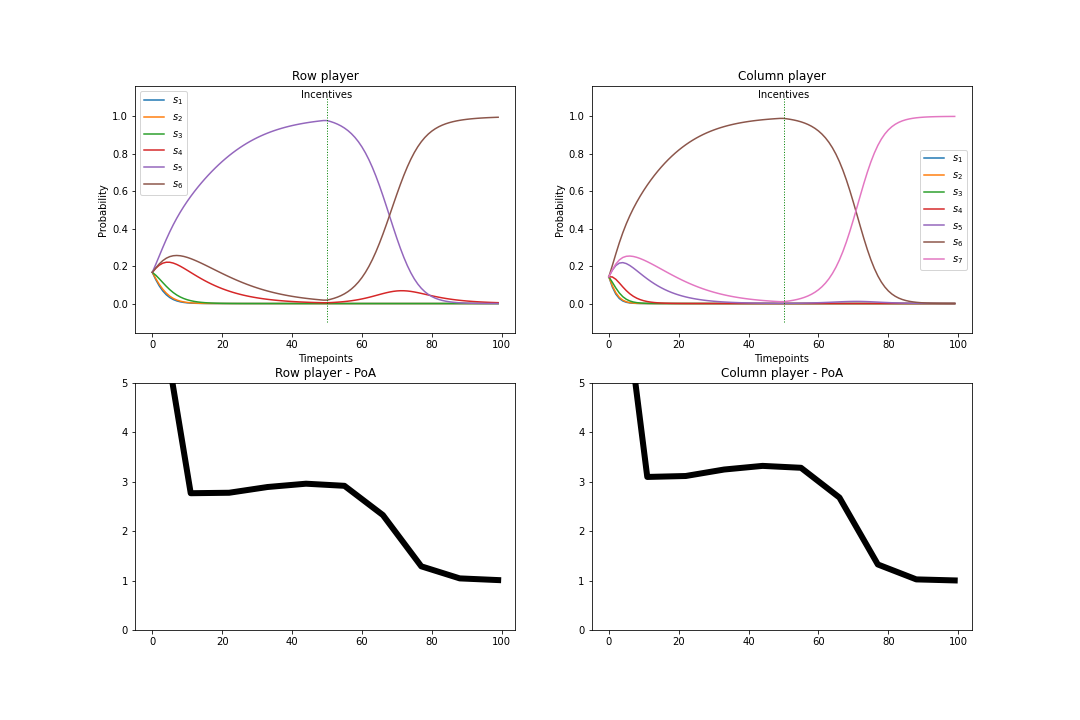
\includegraphics[scale=0.28]{Bin/ARD_penalty_game.png}
    
\end{frame}


\begin{frame}
    \centering
    \Huge{
    ``Targeted incentivisation of behaviours can help escape learned inefficiencies''
    }
\end{frame}
